\section{Introduction}\label{SecIntro}

With the emergence of a new generation of trusted personal devices
(mobile phones, PDAs, smart cards \emph{etc.}), the demand for
techniques to guarantee application security has become even more
prominent. A usual approach is to monitor
executions with a security automaton~\cite{Schneider99}. Upon entry
or exit of a security-critical method, the security automaton updates
its internal state. If it reaches an ``illegal'' state, the
application will be stopped and a security violation will be
reported. This approach is in particular suited for properties that
are expressed as sequences of legal method calls, such as life cycle
properties, or constraints that express how often or under which
conditions a method can be called.
%
However, such a monitoring approach is not always suited due to the
nature and use of certain applications.
Instead, for such applications statical means to enforce security are necessary.
% A commonly advocated approach is to require that the application carries a
% correctness proof with it, which can be validated before installing the
% application on the device. In such a proof carrying code scenario~\cite{Necula97},
% the application provider is required to create this proof.

Security experts typically express security requirements by a collection of
security automata or temporal logic formulae. However, typical program
verification tools use a Hoare logic style for the specifications
(\emph{i.e.}, pre- and postconditions).
Therefore, as a first step towards static
verification of such security properties, this paper proposes a
translation from security properties expressed as an automaton (or a
safety temporal logic formula, which can be translated into an
automaton~\cite{Wolper01}) into program annotations.
We work with Java programs.

The translation described in this paper is defined in several
steps. For each step we provide a correctness proof.
\begin{inparaenum}[(\itshape i\upshape)]
\item We translate a \emph{partial automaton}, to a \emph{total automaton}
that contains a special trap to model that an error has occurred.
% Often it is much more intuitive to specify a security property by a partial
% automaton, (this avoids cluttering up the automaton with transitions that
% \emph{``go wrong''}), while for many tools and algorithms, a complete
% automaton is easier to handle.
We show that the behaviour of a program that is monitored with a partial
automaton is equivalent to the behaviour of a program that is monitored with
the completed automaton.
\item Using an extension of JML~\cite{LeavensPCCRCK05}, we generate annotations
that capture the behaviour of the total automaton. For this, we
generate special method-level set-annotations that are evaluated upon
entry or exit of a method.
We show that run-time monitoring of the program only throws a (new) exception
to signal an annotation violation if the monitor reaches the trap state.
\item We inline the set-annotations from the method specification
to the method body and prove equivalence of the run-time checking behaviour.
\end{inparaenum}
All results in the paper have been established formally using
the PVS theorem prover~\cite{OwreRRSS96}. The complete formalisation
is available via \url{http://www.cs.ru.nl/~tamalet/}.

\psfrag{s1}{\tiny{\(s_1\)}}
\psfrag{s2}{\tiny{\(s_2\)}}
\psfrag{exit(sendSMS)? true -> n := n + 1;}
{\begin{tabular}{l}
\tiny{\exit(\texttt{SendSMS})?\ttt\(\rightarrow\)}\vspace*{-.8em}\\
\tiny{\texttt{n := n + 1};}
\end{tabular}}
\psfrag{exitE(sendSMS)? true -> ;}
{\begin{tabular}{l}
\tiny{\excexit(\texttt{sendSMS})?\ttt \(\rightarrow\)}%\vspace*{-.8em}\\
\tiny{\actskip;}
\end{tabular}}
\psfrag{exit(reset)? true -> n := 0;}
{\begin{tabular}{l}
\tiny{\exit(\texttt{reset})?\ttt \(\rightarrow\)}\vspace*{-.8em} \\
\tiny{\texttt{n :=} 0;}
\end{tabular}}
\psfrag{entry(sendSMS)? n < N -> ;}
{\begin{tabular}{l}
\tiny{\entry(\texttt{sendSMS})? \texttt{n} \(<\) \texttt{N} \(\rightarrow\)} %\vspace*{-.8em} \\
\tiny{\actskip;}
\end{tabular}}
\begin{figure}[t]
\begin{center}
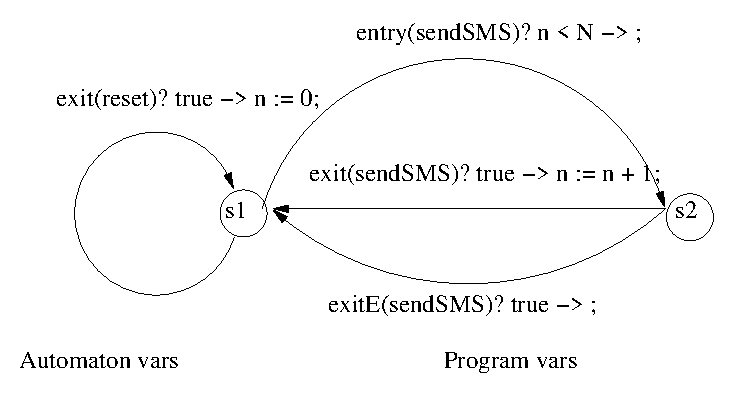
\epsfig{file=limited_sms.eps, width=5.5cm}
\end{center}
\caption{Example Security Automaton}\label{FigExample}
\end{figure}

Throughout this paper, we use a simple example property to
illustrate the different translations: the method \texttt{sendSMS} can
be called and terminate successfully at most \(N\) times in between
calls to a \texttt{reset} method (notice that the counter is not
increased upon exceptional termination of
\texttt{sendSMS}, and that we assume that \texttt{reset} cannot be
called from within \texttt{sendSMS}). Figure~\ref{FigExample} shows a
security automaton that can be used to monitor this property (where
\(\epsilon\) denotes a skip action). Even though very basic,
this example is representative of a wide range of important
resource-related security properties.

The remainder of this paper is organised as follows.
Section~\ref{SecMVA} formalises the automaton format that we
use and defines completion. Next,
Section~\ref{SecProgram} defines the semantics of monitored and
annotated programs. Then Section~\ref{SecAnnotGen} presents the
different translation steps and proves their
correctness. Section~\ref{SecRelated} discusses related work, while
Section~\ref{SecConcl} concludes and discusses future work.
